\usepackage{extras}
\usetheme{default}
\usecolortheme{dove}

\title{Konstruktion av en autonom undsättningsrobot}
\subtitle{Kandidatprojekt i elektronik vid Linköpings universitet}
\author{Grupp 4}
\beamertemplatenavigationsymbolsempty
\date{\today}

\begin{document}

\begin{frame}
  \titlepage
\end{frame}

\begin{frame}[fragile]{PigBot}{Grupp 4}
Syfte och uppgift:
  \begin{itemize}
    \item[-] Undsättningsrobot på prototypnivå
    \item[-] Utforska en labyrint autonomt
    \item[-] Identifiera och undsätta en nödställd
  \end{itemize}
\end{frame}

\begin{frame}{PigBot}{Grupp 4}
  \begin{columns}
    \begin{column}{0.5\textwidth}
      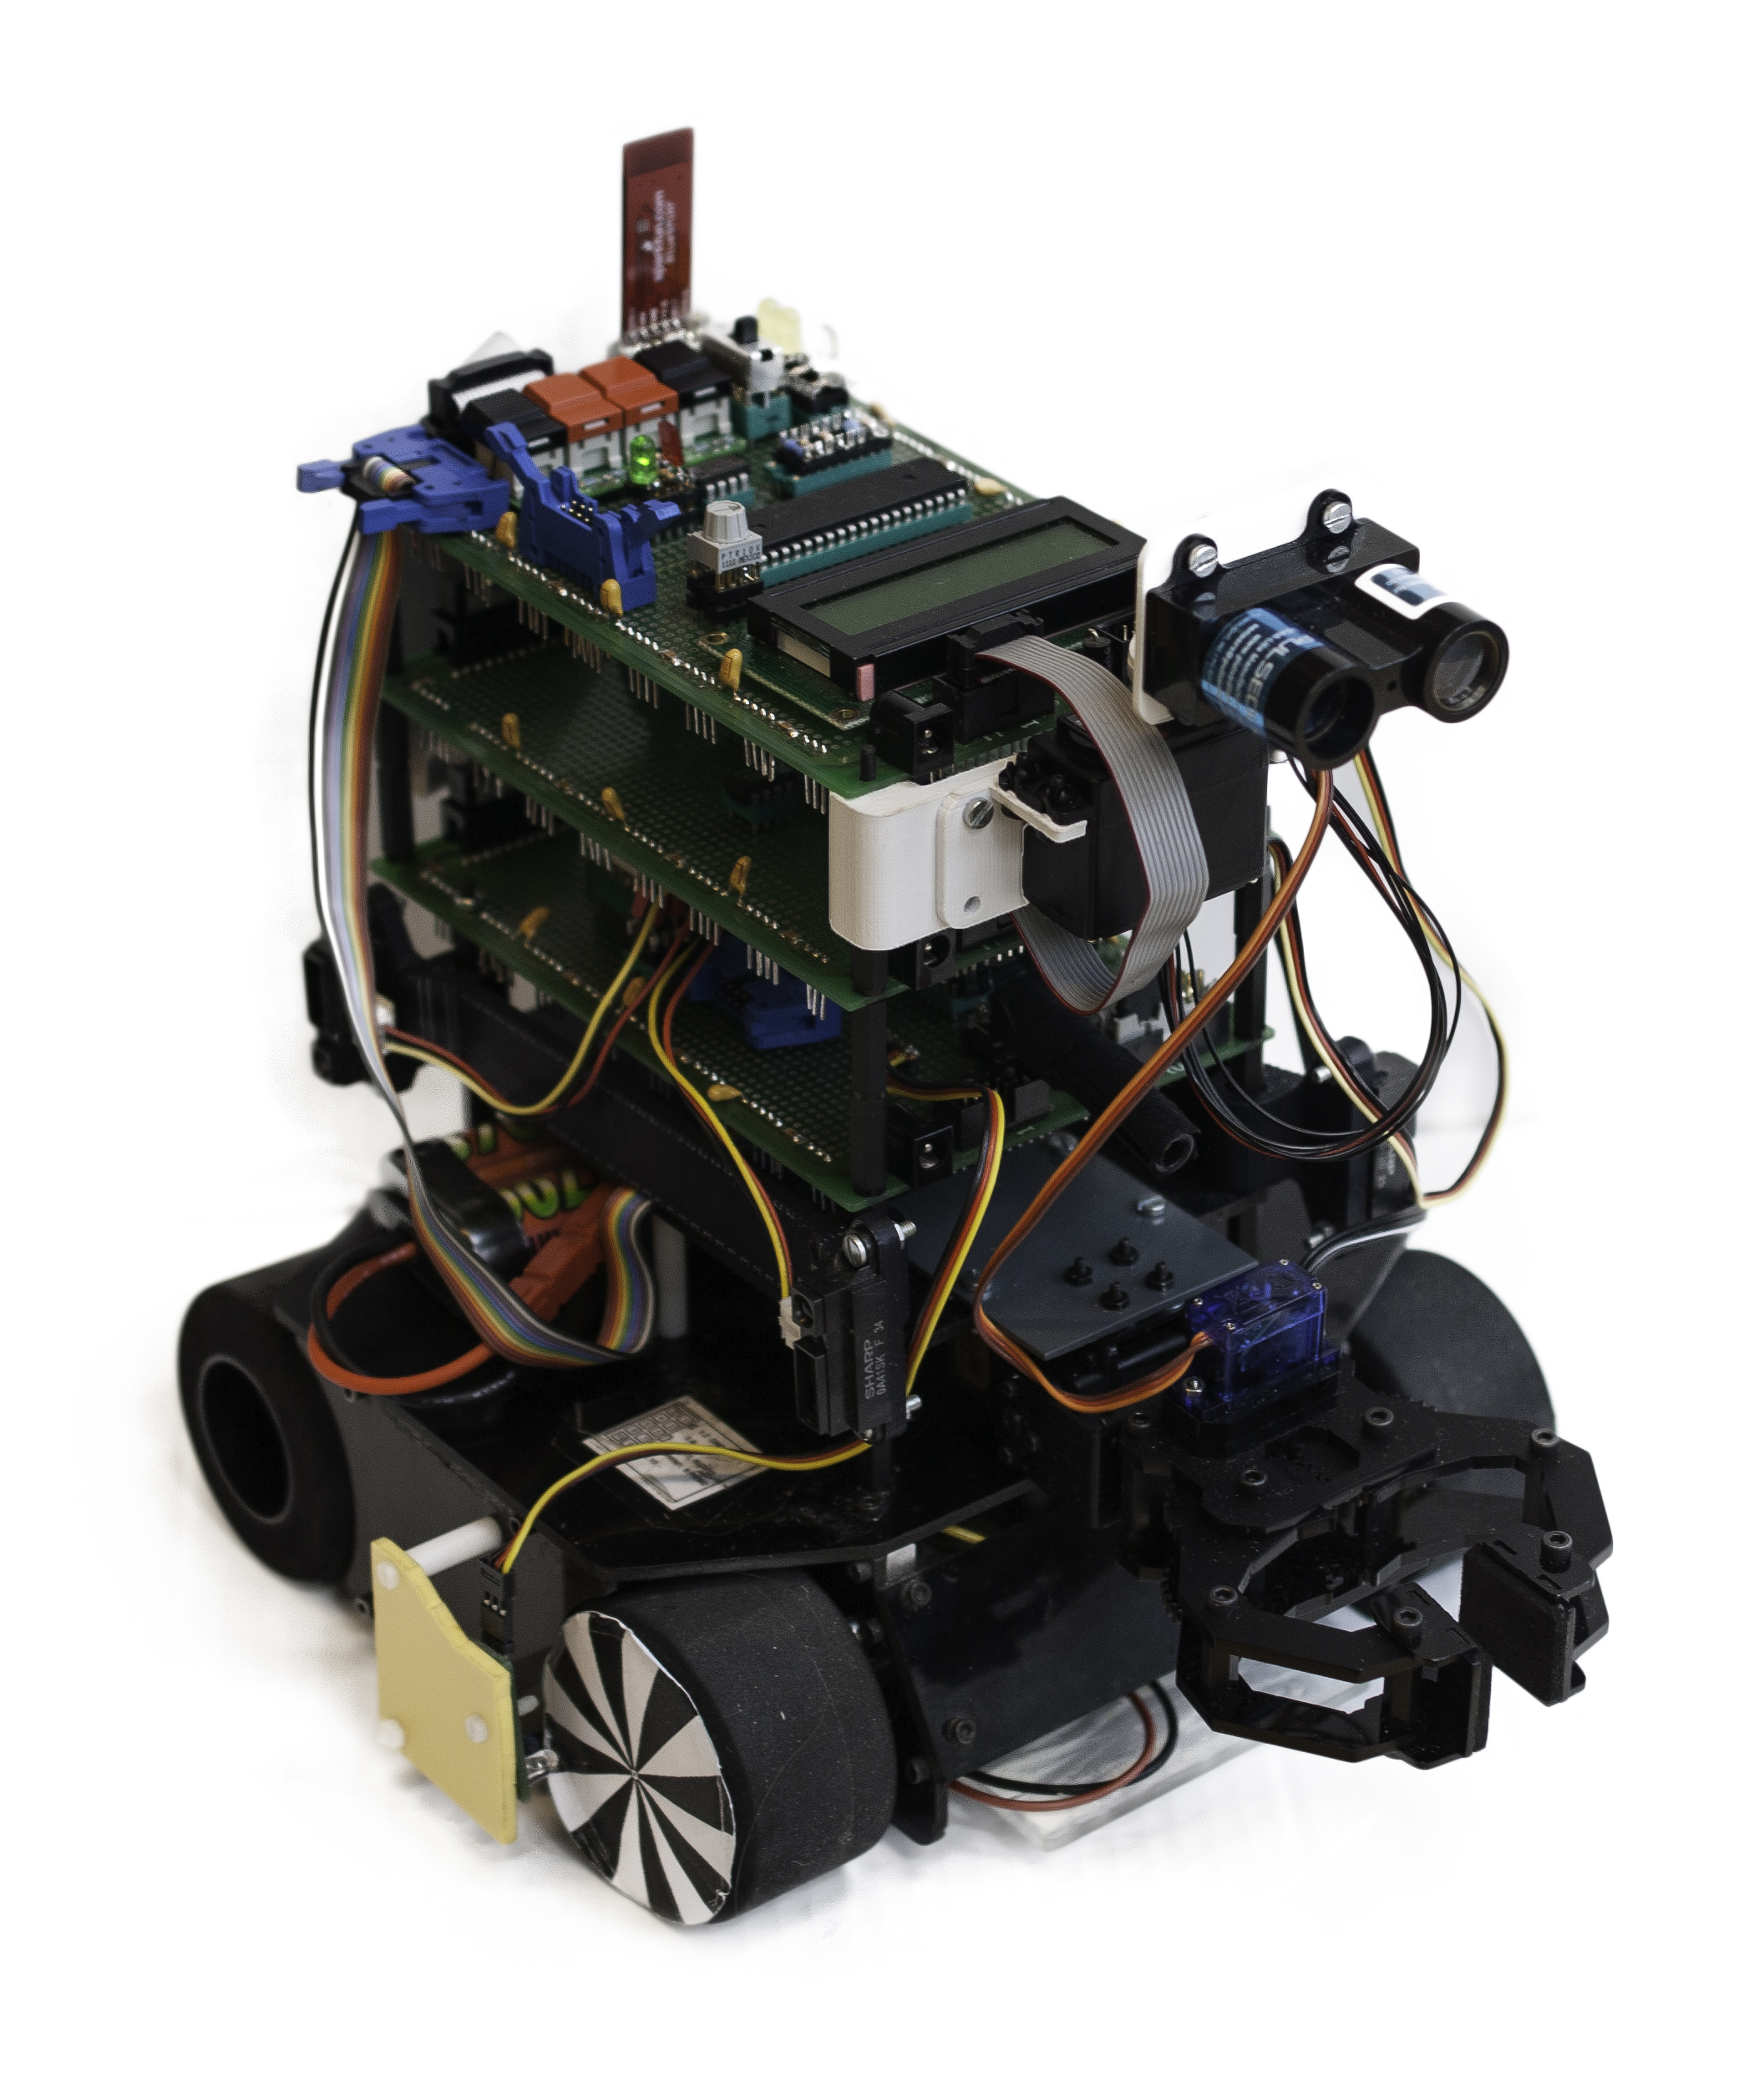
\includegraphics[width=0.9\textwidth]{images/RobotFront.pdf}
    \end{column}
    \begin{column}{0.5\textwidth}
      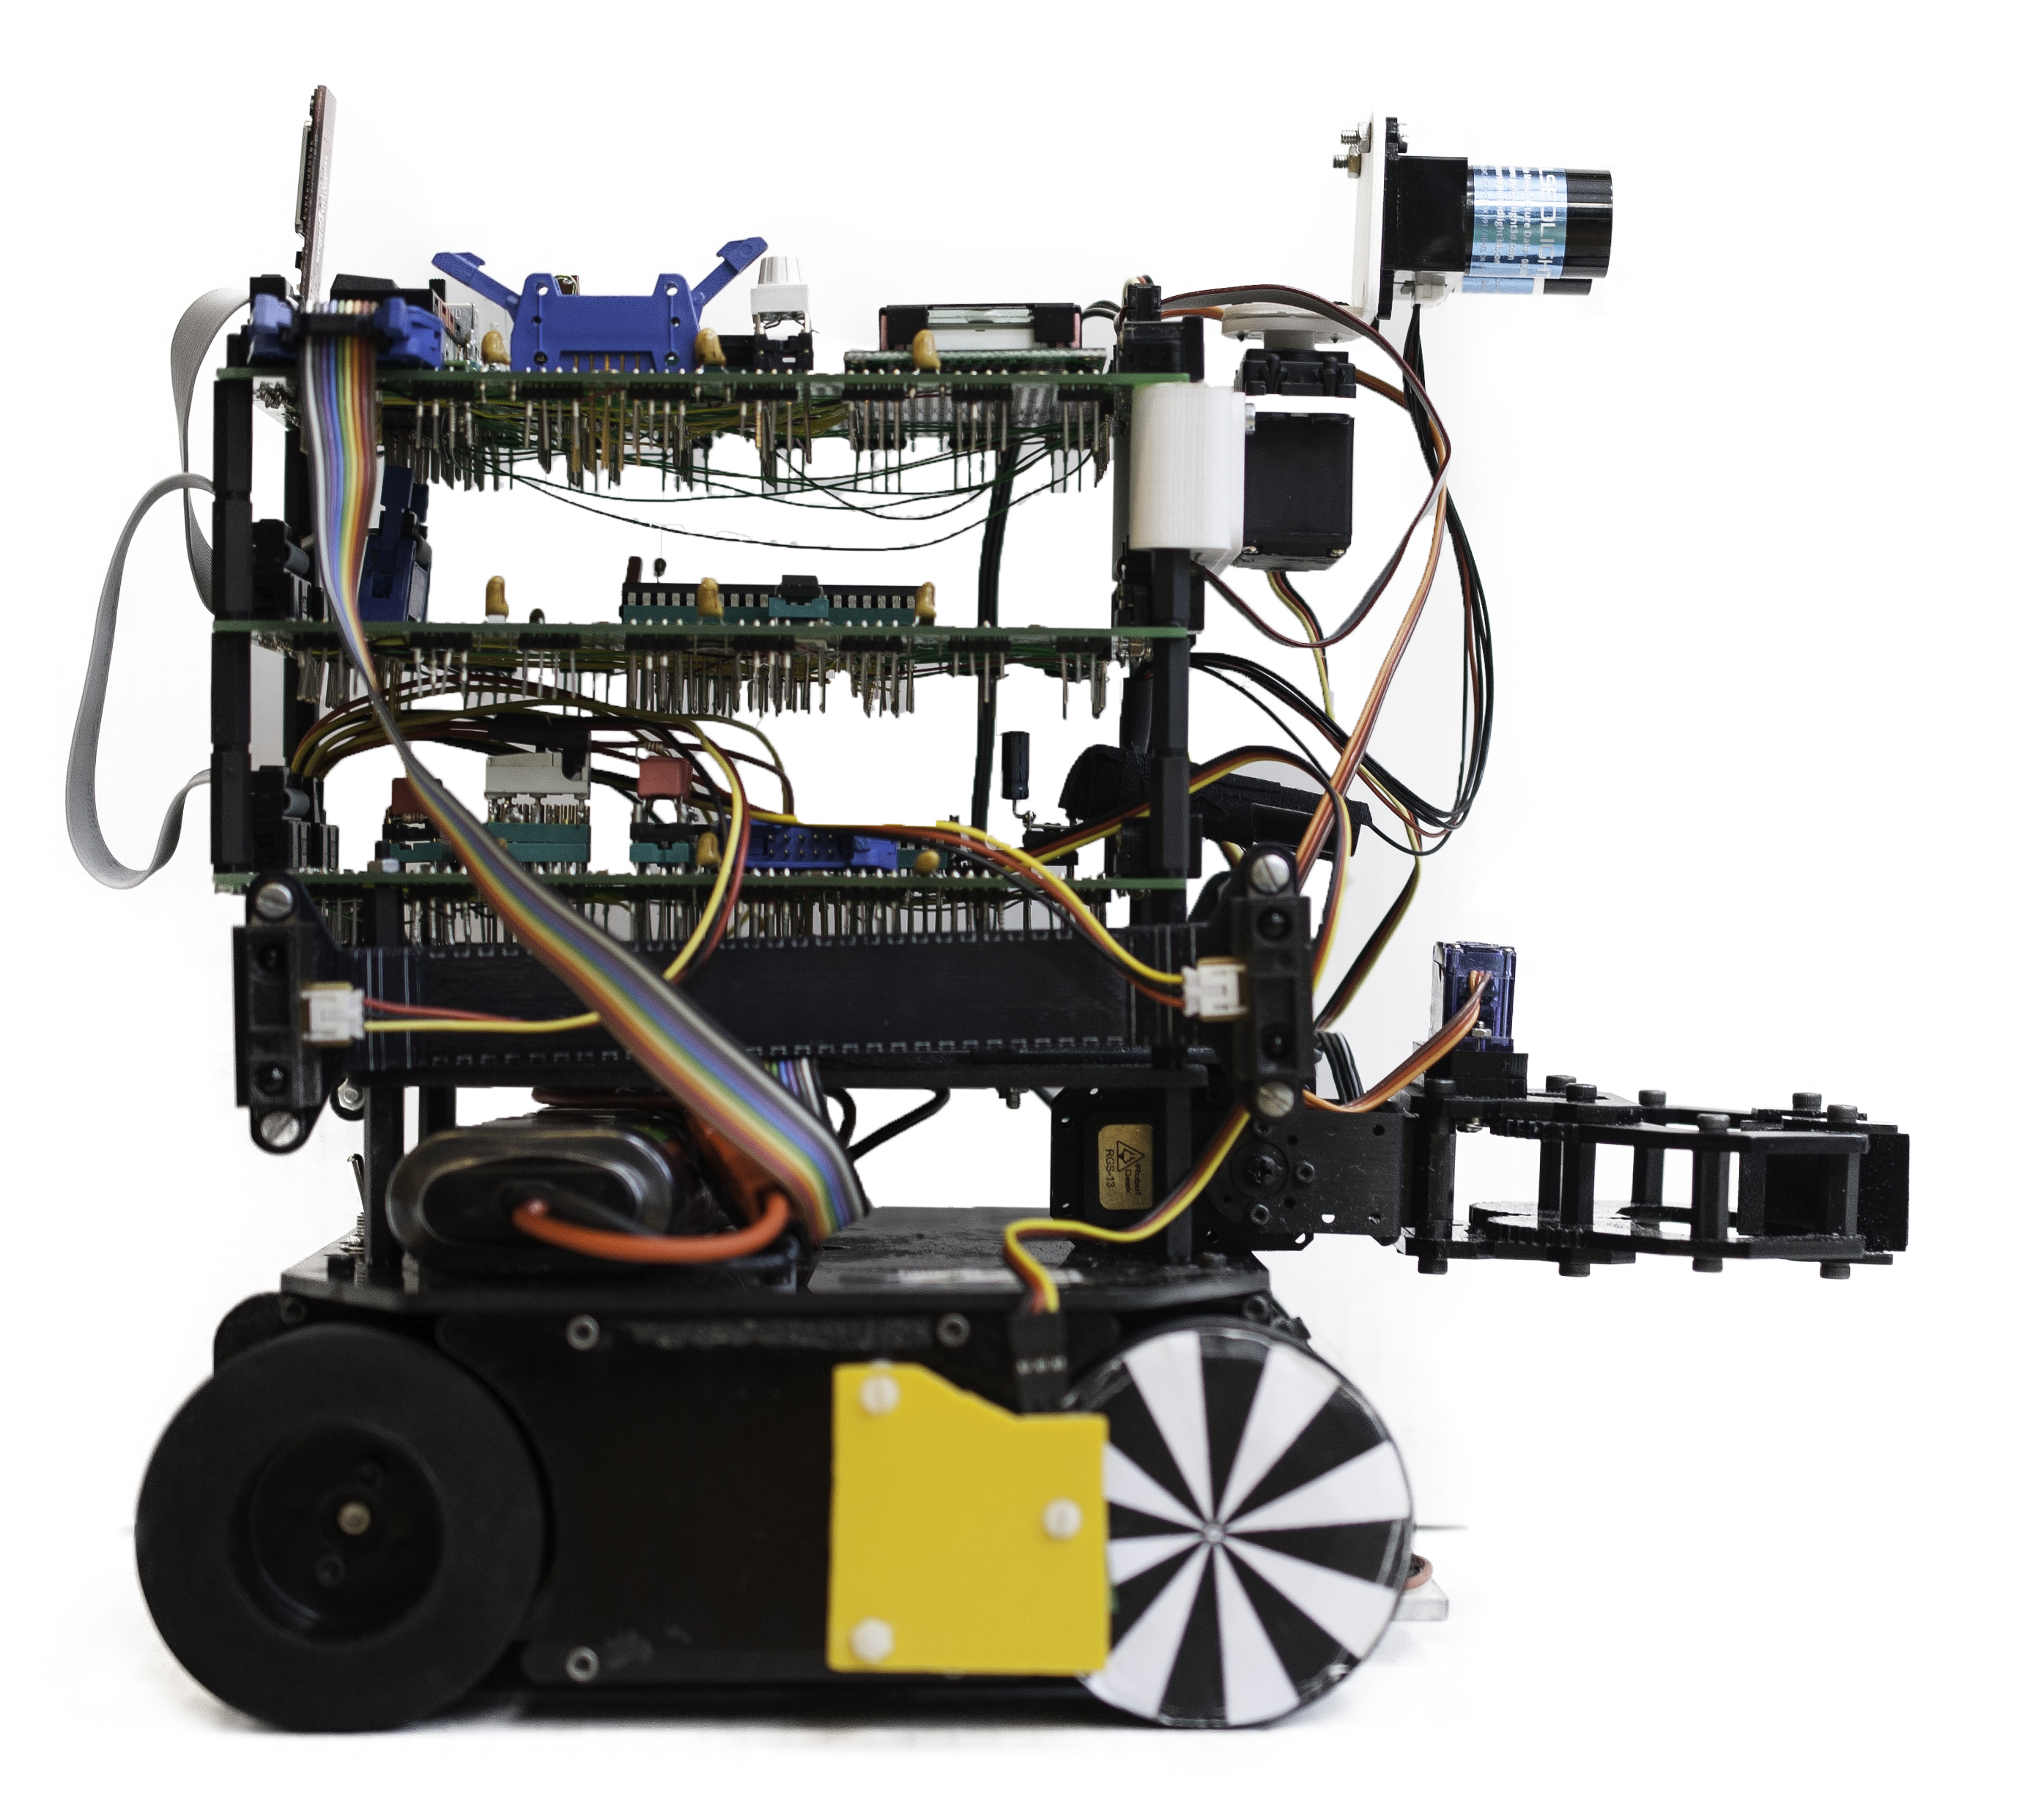
\includegraphics[width=\textwidth]{images/RobotSide.pdf}
    \end{column}
  \end{columns}
\end{frame}

\begin{frame}[fragile]{PigBot}{Grupp 4}

PigBot är upbyggd av moduler, vardera med följande funktion:
  \begin{itemize}
    \item[-] Sensormodul - tar emot och koverterar data från robotens samtliga sensorer
    \item[-] Huvudmodul - ansvarar kommunikationen mellan de olika modulerna samt tar navigeringsbeslut
    \item[-] Styrmodul - sköter reglering av roboten
  \end{itemize}
\end{frame}

\begin{frame}[fragile]{PigBot}{Grupp 4}
\centering
    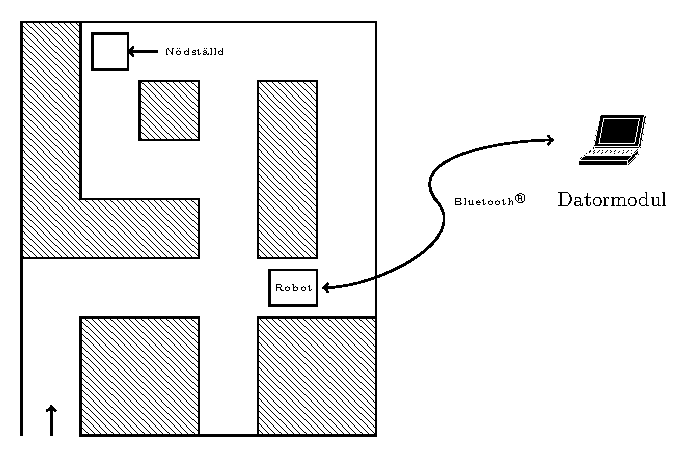
\includegraphics[scale=0.7]{images/overview.pdf}
\end{frame}

%Start förstudie

\begin{frame}{Förstudie}{Grupp 4 - PigBot}
Förstudie
\pause
  \begin{itemize}
    \item[-] En regleruppgift
    \item[-] En sensoruppgift 
    \item[-] En kommunikations/konstruktionsuppgift
  \end{itemize}
\end{frame}

%%%

\begin{frame}{Förstudie}{Grupp 4 - PigBot}
Frågeställningar regleruppgift
  \begin{itemize}
\pause
    \item[-] Reglering
\pause
\begin{itemize}
	\item [-] Hur kan man reglera en robot så att den kör rakt i en korridor?
	\item [-] Hur kan styrning ske i kurvor och under rotationer?
\end{itemize}
\pause
    \item[-] Kartläggning och optimering 
\begin{itemize}
	\item [-] Hur kan en robot som enbart har tillgång till sensordata kartlägga en okänd labyrint?
	\item [-] Vilka kartsökningsalgoritmer ger en effektiv avsökningssekvens av en okänd labyrints korridorer?
	\item [-] Givet en karta över en labyrint, hur kan då den kortaste vägen mellan två punkter beräknas?
\end{itemize}
  \end{itemize}
\end{frame}

%%

\begin{frame}{Förstudie}{Grupp 4 - PigBot}
Resultat regleruppgift
\pause
  \begin{itemize}
    \item[-] Reglering
\begin{itemize}
	\item [-] PID-reglering
\end{itemize}

    \item[-] Kartläggning och vägoptimering
\begin{itemize}
	\item [-] Kalmanfilter
	\item [-] Högerväggföljning
\end{itemize}
  \end{itemize}
\end{frame}

%%

\begin{frame}{Förstudie}{Grupp 4 - PigBot}
Frågeställningar sensoruppgift
\pause
\begin{itemize}
    \item[-] Vilka sensorer finns det som stöd för att roboten ska kunna utföra sitt uppdrag? Hur fungerar dessa? Finns det olika typer?
    \item[-] Vilka sensorer är lämpliga att använda till projektet?
    \item[-] Hur kan dessa implementeras?
\end{itemize}
\end{frame}

%%

\begin{frame}{Förstudie}{Grupp 4 - PigBot}
Resultat sensoruppgift
  \begin{itemize}
\pause
    \item[-] Gav konkreta förslag gällande vilka sensorer som roboten borde använda 
  \end{itemize}
\end{frame}

%%
\begin{frame}{Förstudie}{Grupp 4 - PigBot}
Frågeställningar kommunikationsuppgift
\pause
\begin{itemize}
	\item[-] Vilken busstyp är lämpligast, SPI eller I\textsuperscript{2}C, och hur ska den konfigureras?
	\item[-] Vilka för- och nackdelar finns med C repektive Assembler? 
	\item[-] Hur ska tester designas?
	\item[-] Vad är viktiga faktorer att ha i åtanke vid design av modulbaserade projekt?
\end{itemize}
\end{frame}

%%

\begin{frame}{Förstudie}{Grupp 4 - PigBot}
Resultat kommunikationsuppgift
\pause
\begin{itemize}
	\item[-] I\textsuperscript{2}C-buss med kommunikationsmodul som masterenhet
	\item[-] C-koden prioriterades framför assembler
	\item[-] Genom debugging samt test av hårdvara med hjälp av logikanalysatorn
	\item[-] Uppdelning av moduler innebär ett flertal fördelar, men tänk på systemet i sin helhet
\end{itemize}
\end{frame}

%Slut förstudie

% Olles del
\begin{frame}{Sensormodul}{Grupp 4 - PigBot} 
  \begin{columns}
    \begin{column}{0.5\textwidth}
      \centering
      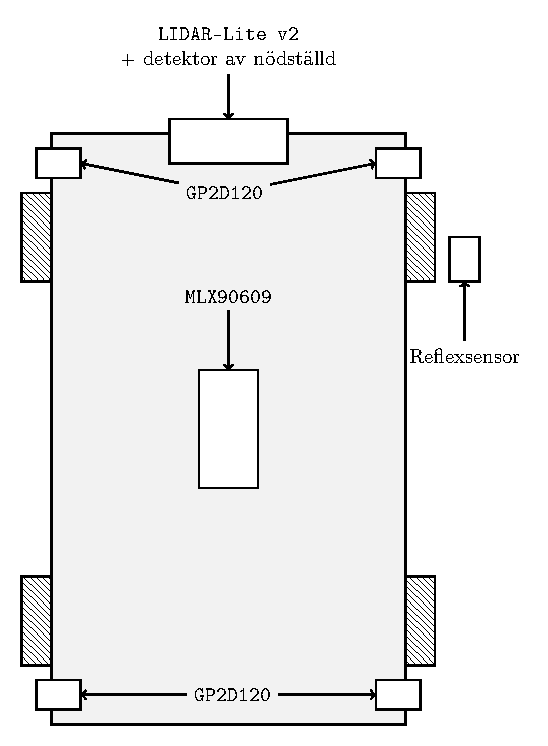
\includegraphics[scale=0.6]{images/sensor.pdf}
    \end{column}
    \begin{column}{0.5\textwidth}
      \begin{itemize}
	\item[-] Åtta sensorer
	  \begin{itemize}
	    \item[-] Fyra sidosensorer (IR)
	    \item[-] En främre sensor (laser)
	    \item[-] En reflexsensor (IR)
	    \item[-] Ett gyroskop (SPI)
	    \item[-] En måldetektor (IR)
	  \end{itemize}
	  \pause
	\item[-] Beräknar median efter sampling
	  \pause
	\item[-] Skickar vidare i $30$ Hz
      \end{itemize}
    \end{column}

  \end{columns}
\end{frame}

\begin{frame}{Huvudmodul}{Grupp 4 - PigBot}
  \begin{center}
    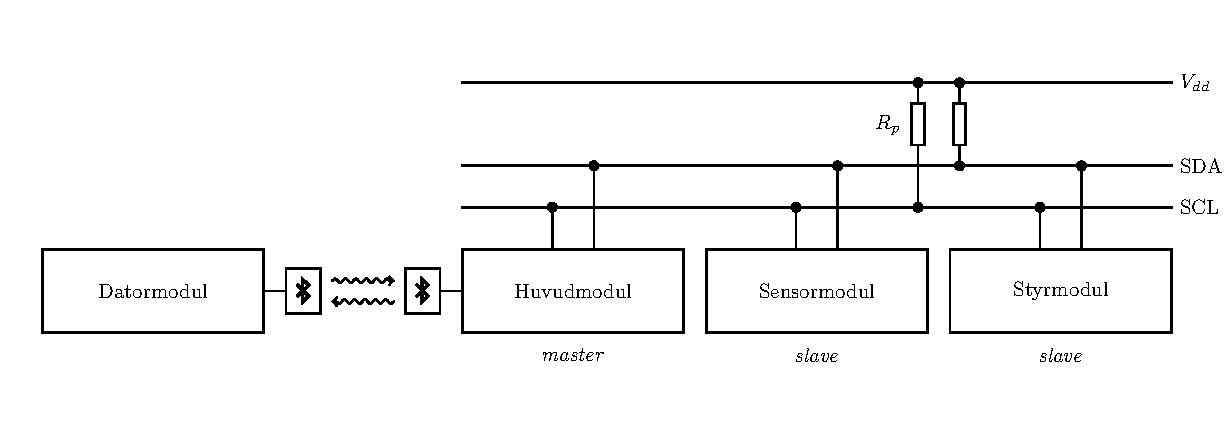
\includegraphics[scale=0.5]{images/communication.pdf} 
    \pause
    \begin{longtable}{c c c c c}
      {Identifierare} & & {Kommando} & & {Data} \\ \hline
      246-255 & $\rightarrow$ & 0-245 & $\rightarrow$ & 0-245 
    \end{longtable}
  \end{center}
\end{frame}

\begin{frame}{Huvudmodul}{Grupp 4 - PigBot}
  \begin{itemize}
    \item[-] Högerföljning och dead-end-filling
    \item[-] A*
  \end{itemize}
  \pause
  \begin{columns}
    \begin{column}{0.45\textwidth}
      \centering
      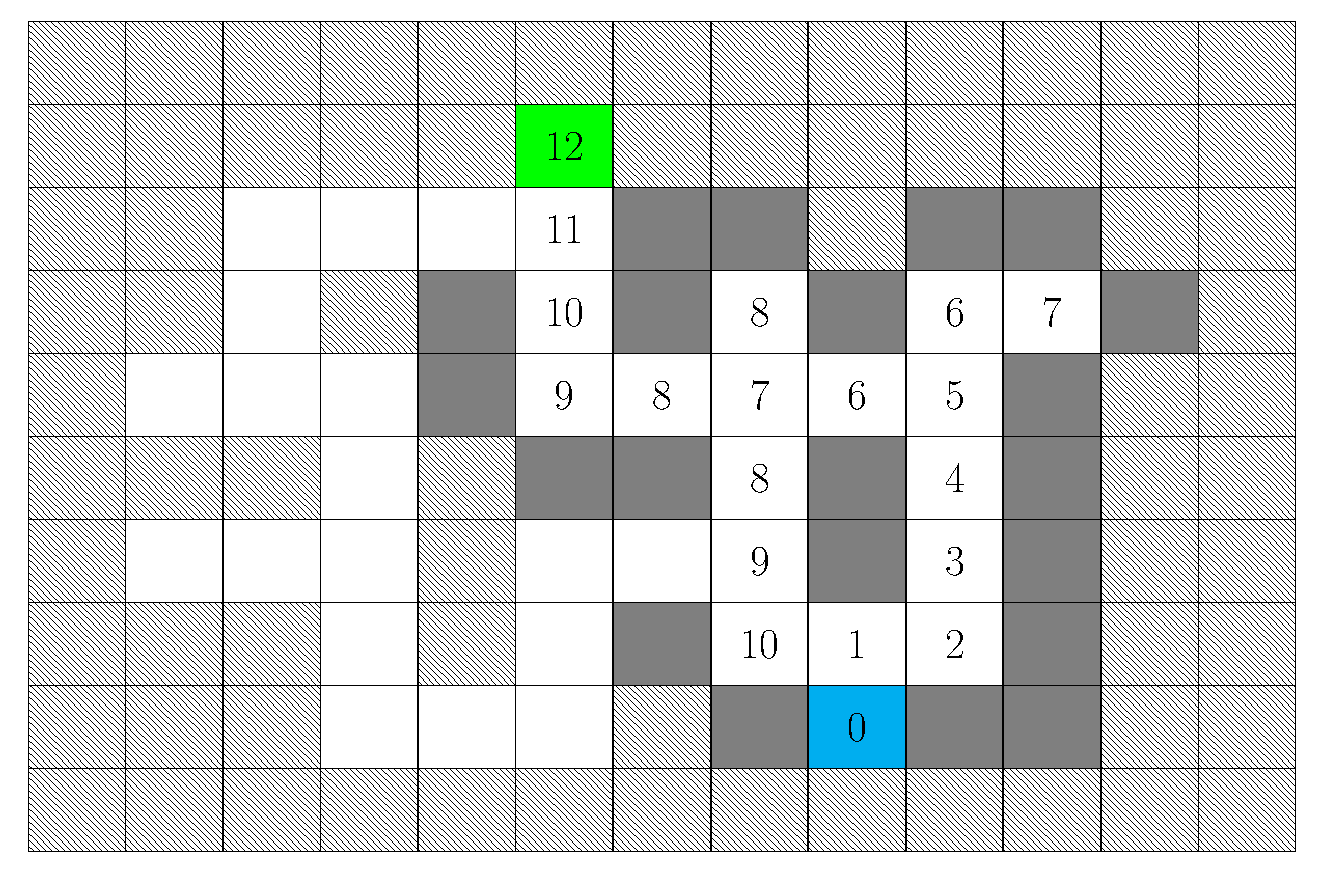
\includegraphics[width=\textwidth]{images/map.pdf}
    \end{column}
    \begin{column}{0.1\textwidth}
      \centering
      $\rightarrow$
    \end{column}
    \begin{column}{0.45\textwidth}
      \centering
      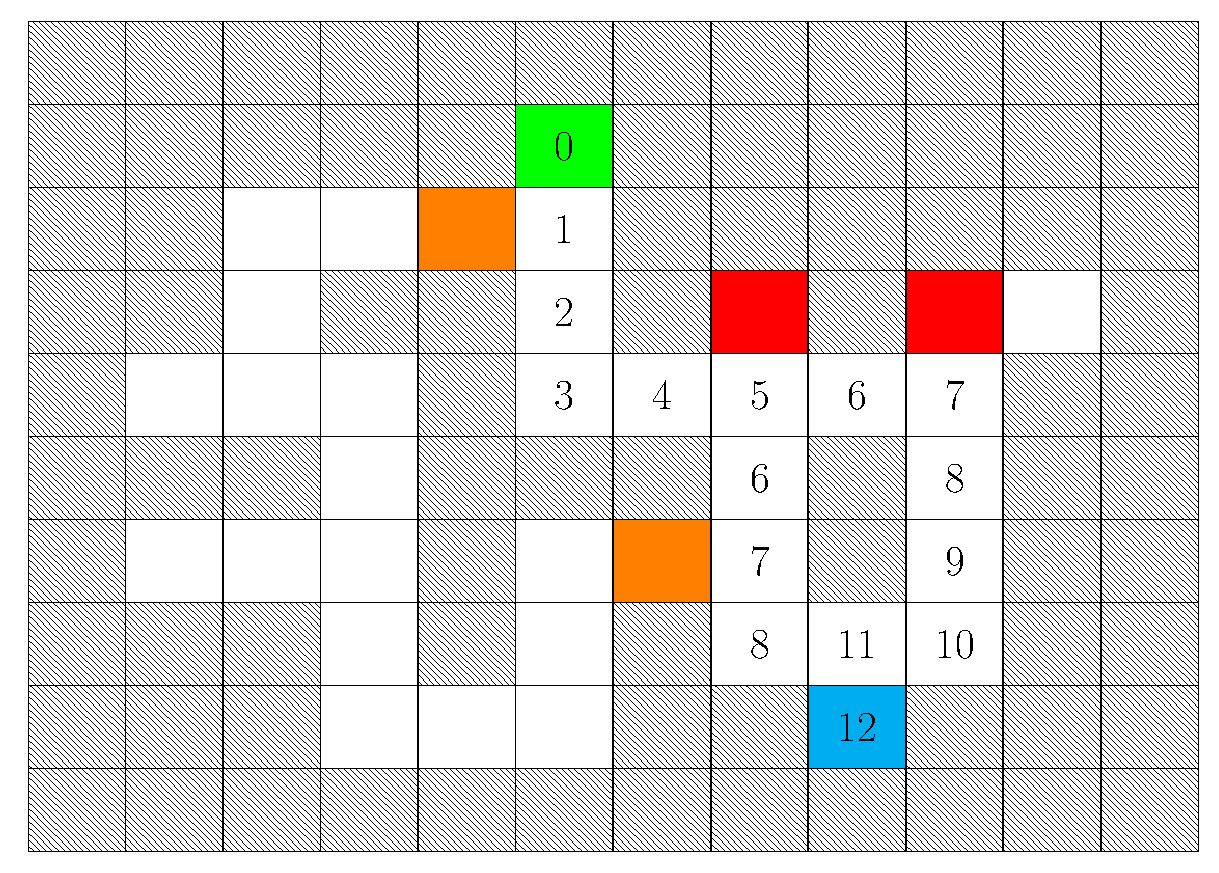
\includegraphics[width=\textwidth]{images/path.pdf}
    \end{column}
  \end{columns}
\end{frame}


% Isaks del
\begin{frame}{PigBot}{Grupp 4}
	\begin{columns}
		\begin{column}{0.5\textwidth}
			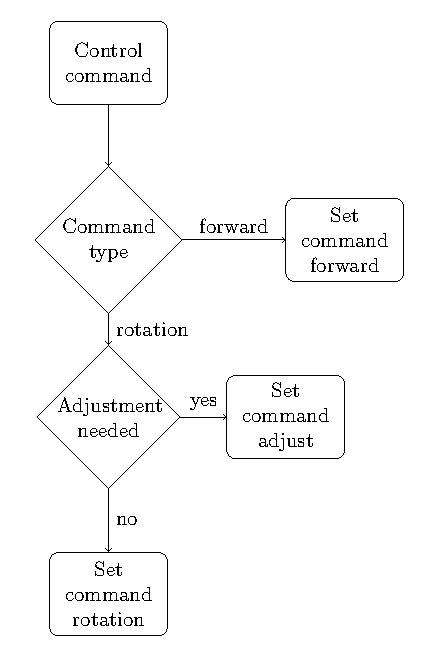
\includegraphics[width=0.9\textwidth]{images/controllerControlFlow.pdf}
		\end{column}
		\pause
    		\begin{column}{0.5\textwidth}
      			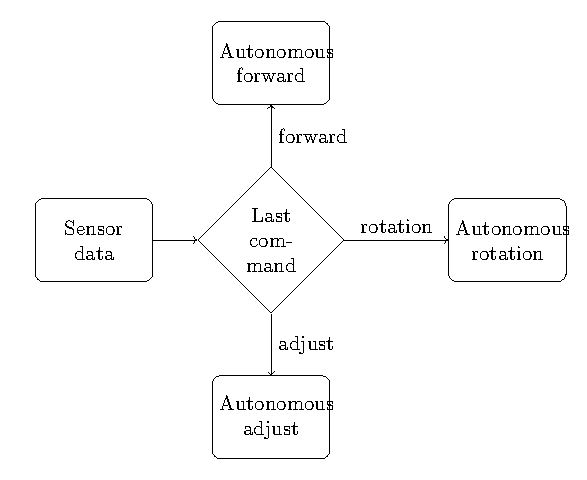
\includegraphics[width=\textwidth]{images/controllerSensorFlow.pdf}
    		\end{column}
  	\end{columns}
\end{frame}

\begin{frame}{PigBot}{Grupp 4}
\centering
	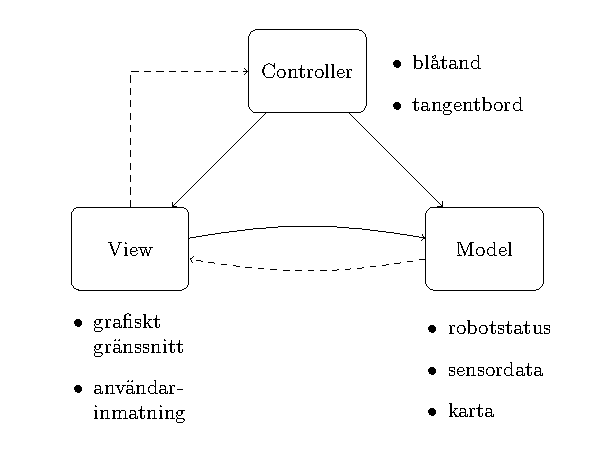
\includegraphics[width=0.9\textwidth]{images/modelViewController.pdf}
\end{frame}

\begin{frame}{PigBot}{Grupp 4}
	\begin{tikzpicture}[scale=0.135]
		\pgftext{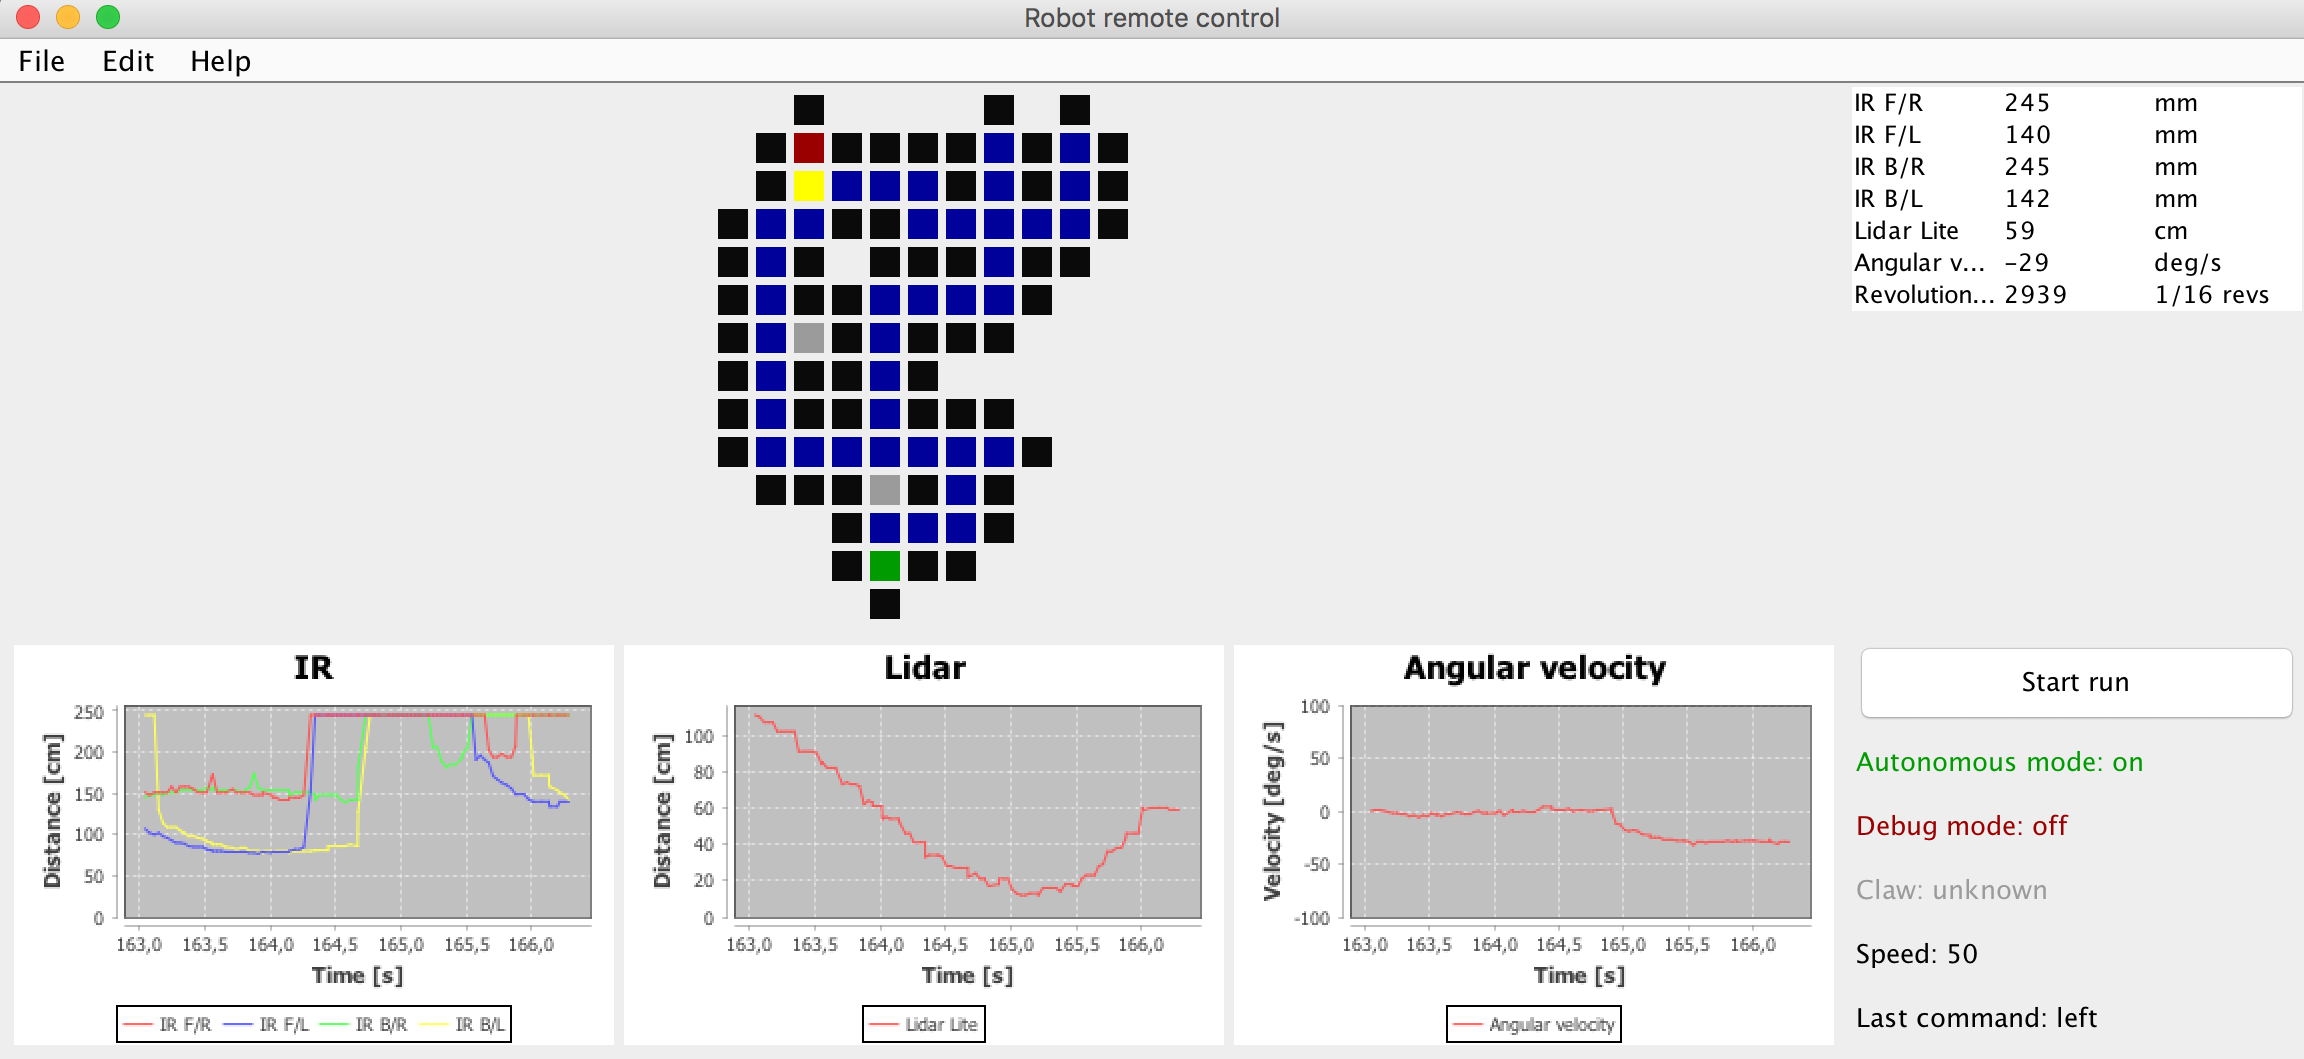
\includegraphics[width=2304pt]{images/computerModule.png}} at (0pt,0pt);
		\fill<3-6>[black, opacity = 0.7] (-1150 pt, 527pt) rectangle (1150pt , 450pt);
		\fill<2, 4-6>[black, opacity = 0.7] (-1150pt, 450pt) rectangle (700pt , -100pt);
		\fill<2-4, 6>[black, opacity = 0.7] (-1150pt, -100pt) rectangle (700pt , -527pt);
		\fill<2-3, 5-6>[black, opacity = 0.7] (700pt, 450pt) rectangle (1150pt , -100pt);
		\fill<2-5>[black, opacity = 0.7] (700pt, -100pt) rectangle (1150pt , -527pt);
	\end{tikzpicture}
\end{frame}


\begin{frame}{Resultat}{Grupp 4 - PigBot}

  \begin{itemize}
    \item[-] Roboten PigBot
    \item[-] Prestanda
  \end{itemize}
\end{frame}


\begin{frame}{Resultat}{Grupp 4 - PigBot}
\begin{center}
 \includemedia[
    width=8cm,
    height=8cm,
    activate=pageopen,
    addresource=movies/Robot.MP4,
    flashvars={source=movies/Robot.MP4 &autoPlay=false}
 ]{}{VPlayer.swf}
\end {center}
\end{frame}


\begin{frame}{Utvecklingspotential }{Grupp 4 - PigBot}

  \begin{itemize}
    \item[-] Optimera avsökningsalgoritm
    \item[-] Göra mer verklighetsanpassad
	\begin{itemize}
	  \item Öppna ytor
	  \item Rotation
	\end{itemize}	
    \item[-] Förbättra användarupplevelsen
     	\begin{itemize}
	  \item 3D-karta
	\end{itemize}
   \end{itemize}
\end{frame}


\begin{frame}{Hur har gruppen jobbat?}{Grupp 4 - PigBot}
  \begin{itemize}
\pause
    \item[-] Gruppkontrakt 
\pause
    \item[-] Paruppdelning
\pause
    \item[-] Bestämda mötestider
\pause
    \item[-] Tid och plats
\pause
    \item[-] Umgänge utanför arbetstid
  \end{itemize}
\end{frame}

\begin{frame}{Problemlösning}{Grupp 4 - PigBot}
  \begin{itemize}
 \pause
    \item[-] Situationsanpassat
\pause
    \item[-] Exempel
  \end{itemize}
\end{frame}

\begin{frame}{Konflikter}{Grupp 4 - PigBot}
  \begin{itemize}
 \pause
    \item[-] Kommunikation
\pause
    \item[-] Ansvar
  \end{itemize}
\end{frame}

\begin{frame}{Sammanfattning}{Grupp 4 - PigBot}
  \begin{itemize}
 \pause
    \item[-] Uppnådda mål
 \pause
    \item[-] Engagemang
  \pause
    \item[-] Erfarenhet
  \end{itemize}
\end{frame}

\end{document}
